\section{Search for Top Squark Pair Production in the Single Lepton Final State}
\label{sec:stop}

This section presents the results of a dedicated search for the direct pair production of top squarks, based on an integrated luminosity of 9.7~fb$^{-1}$.
The decay of the top squark depends on the difference between its mass and that of the \lsp\ LSP,
$\Delta m = m_{\tilde{t}}-m_{\lsp}$. If $\Delta m > m_{t}$, the decay $\tilde{t}\to t\lsp$ is expected
to have a large branching fraction. If there is a light chargino \chip, the decay 
$\tilde{t}\to b\chip\to b W \lsp$ is expected to be significant, especially in the $\Delta m < m_{t}$ region.
The pair production of top squarks decaying to either of these channels leads to events with two b-jets, two W bosons,
and \met\ from the invisible LSPs. Our signal thus resembles SM $t\bar{t}$ production but with larger \met\ from
the invisible LSPs.
We focus on the single lepton final state, which has a significant branching fraction due to the two W bosons,
and smaller SM backgrounds than the all-hadronic final state.
We thus select events with a single lepton and jets and discriminate between
signal and background using \met\ and the transverse mass \mt, discussed below.

%\subsection{Event Selection}

We require the presence of exactly one well-identified and isolated lepton (e or $\mu$) with transverse
momentum \pt\ $>$ 30 GeV. 
We select events with at least four jets with \pt\ $>$ 30 GeV,
which must be well-separated from the selected leptons.
At least one of these jets is required to be consistent with coming from the decay of heavy flavor hadrons, as
identified by the Combined Secondary Vertex Medium Point (CSVM) b-tagging algorithm~\cite{ref:btag}.
The jet requirements suppress SM backgrounds from W bosons produced in association with jets from initial state
radiation (ISR), referred to as the \wjets\ background. 
The \met\ is required to exceed 50 GeV, suppressing the background from QCD multijet production.

%\subsection{Backgrounds and Estimation Strategy}

The SM background satisfying the above requirements is dominated by $t\bar{t}$ production where
one W boson decays hadronically and the other leptonically (\ttljets), or where both W bosons decay leptonically (\ttll).
There is a small contribution from \wjets, as well as a variety of rare SM
processes, dominated by $t\bar{t}$ produced in association with a vector boson
($t\bar{t}W$ and $t\bar{t}Z$).

To define signal regions, we require the events to have large transverse mass, defined as:

\begin{equation}
M_T = \sqrt{ 2 p_{T}^{\ell} \met ( 1-cos(\Delta\phi))},
\end{equation}

where $p_{T}^{\ell}$ is the lepton transverse momentum and $\Delta\phi$ is the difference in azimuthal angles between the lepton
and \met. This requirement strongly suppresses the background from \ttljets\ and \wjets, which have a kinematic endpoint
at \mt\ $=$ $M_W$ since the lepton and neutrino (which produces the \met) are produced together in the decay of the W.
For signal events, as well as the \ttll\ background, the presence of more than one invisible
particle in the final state leads to events with \mt\ $>>$ $M_W$. 
In addition to the \mt\ requirement, we make several 
\met\ requirements to achieve sensitivity to signals with different mass spectra.
Signal regions with large (small) \met\ requirements are more sensitive to signals with large (small) values of $\Delta m$.

The dominant background in our signal regions is \ttll, which may produce events with large \met\ and \mt\ due to the presence of
two invisible neutrinos. In order for \ttll\ events to pass the signal region selection, one of the two W leptons must not be identified,
which occurs if it is outside the acceptance, is a hadronic $\tau$ decaying to three charged particles (3-prong decay),
is a hadronic $\tau$ decaying to a single charged particle (1-prong decay), or is an electron or muon that fails the lepton identification
requirements. The latter two categories are suppressed by vetoing events that contain, in addition to the selected lepton, 
a charged particle with \pt\ $>$ 10 GeV that is isolated in space from other energetic charged particles. Furthermore, additional jets 
from initial state or final state radiation (ISR/FSR) are required to satisfy the jet multiplicity requirement $n_{jets}\geq4$. 
To validate and correct the MC modeling of jets from radiation, the MC is compared to data in a dilepton control region dominated by \ttll. The MC distribution of $n_{jets}$ is reweighted to 
match the corresponding data distribution, resulting in corrections of (1--7)\%.

The SM backgrounds are estimated from events simulated with Monte Carlo (MC) techniques, which are validated and 
(if necessary) corrected using comparisons to data in control regions. The MC expectation is normalized to data in the \mt\ peak region,
in order to remove systematic uncertainties from integrated luminosity and $t\bar{t}$ cross section, and then extrapolated to the 
large \mt\ region. Correction factors and corresponding systematic uncertainties on the MC extrapolation factors are evaluated by 
comparing MC to data in dedicated control regions dominated by \wjets\ (obtained by vetoing events with b-jets), \ttll\ 
(obtained by requiring two selected leptons), and a mixture of \ttll\ and \ttljets\ (obtained by requiring a selected lepton and 
an isolated track). The dominant systematic uncertainty in the background prediction is due to the limited statistical precision in
the data control samples used for these tests.


	\begin{table}[!h]																															
	\begin{center}																															
	{\footnotesize																															
	\begin{tabular}{l||c|c|c|c|c|c|c}																															
	\hline																															
	Sample		&	SRA			&	SRB			&	SRC			&	SRD			&	SRE			&	SRF			&	SRG\\				
	\hline																															
	\hline																															
	\multicolumn{8}{c}{Muon}	\\																														
	\hline																															
	\ttdl\  		&$	330.6	\pm	21.9	$&$	183.4	\pm	20.7	$&$	59.5	\pm	10.0	$&$	22.5	\pm	6.2	$&$	9.0	\pm	3.9	$&$	3.7	\pm	1.8	$&$	2.2	\pm	1.2	$	\\
	\ttsl\ \& single top (1\Lep) 		&$	92.8	\pm	27.5	$&$	41.0	\pm	8.6	$&$	11.5	\pm	3.5	$&$	7.7	\pm	3.4	$&$	0.7	\pm	0.6	$&$	0.3	\pm	0.2	$&$	0.2	\pm	0.2	$	\\
	\wjets\ 		&$	19.2	\pm	4.5	$&$	10.0	\pm	2.2	$&$	3.1	\pm	1.0	$&$	1.2	\pm	0.6	$&$	0.6	\pm	0.4	$&$	0.4	\pm	0.3	$&$	0.2	\pm	0.2	$	\\
	Rare 		&$	33.2	\pm	16.6	$&$	22.7	\pm	11.4	$&$	9.0	\pm	4.5	$&$	4.8	\pm	2.4	$&$	2.9	\pm	1.5	$&$	1.2	\pm	0.6	$&$	1.0	\pm	0.5	$	\\
	\hline																															
	Total 		&$	475.8	\pm	37.8	$&$	257.2	\pm	24.2	$&$	83.2	\pm	11.3	$&$	36.2	\pm	7.4	$&$	13.3	\pm	4.2	$&$	5.5	\pm	1.9	$&$	3.6	\pm	1.3	$	\\
	\hline																															
	\hline																															
	Data 		&$	?			$&$	?			$&$	?			$&$	?			$&$	?			$&$	?			$&$	?			$	\\
	\hline																															
	\hline																															
	\hline																															
	\multicolumn{8}{c}{Electron}	\\																														
	\hline																															
	\ttdl\  		&$	248.1	\pm	16.9	$&$	144.4	\pm	16.6	$&$	51.1	\pm	8.8	$&$	16.2	\pm	4.6	$&$	5.5	\pm	2.5	$&$	2.5	\pm	1.3	$&$	1.3	\pm	0.7	$	\\
	\ttsl\ \& single top (1\Lep) 		&$	68.0	\pm	20.2	$&$	31.2	\pm	6.6	$&$	9.3	\pm	2.8	$&$	4.9	\pm	2.1	$&$	0.5	\pm	0.4	$&$	0.2	\pm	0.2	$&$	0.2	\pm	0.2	$	\\
	\wjets\ 		&$	14.3	\pm	3.3	$&$	7.5	\pm	1.7	$&$	2.4	\pm	0.8	$&$	0.8	\pm	0.4	$&$	0.4	\pm	0.3	$&$	0.3	\pm	0.2	$&$	0.1	\pm	0.2	$	\\
	Rare 		&$	25.8	\pm	12.9	$&$	15.8	\pm	7.9	$&$	7.1	\pm	3.6	$&$	2.9	\pm	1.5	$&$	0.7	\pm	0.4	$&$	0.3	\pm	0.2	$&$	0.1	\pm	0.1	$	\\
	\hline																															
	Total 		&$	356.2	\pm	28.4	$&$	198.9	\pm	19.0	$&$	69.9	\pm	9.7	$&$	24.7	\pm	5.3	$&$	7.1	\pm	2.5	$&$	3.4	\pm	1.3	$&$	1.7	\pm	0.8	$	\\
	\hline																															
	\hline																															
	Data 		&$	?			$&$	?			$&$	?			$&$	?			$&$	?			$&$	?			$&$	?			$	\\
	\hline																															
	\hline																															
	\hline																															
	\multicolumn{8}{c}{Muon+Electron Combined}		\\																													
	\hline																															
	\ttdl\  		&$	578.7	\pm	38.1	$&$	327.8	\pm	36.6	$&$	110.6	\pm	18.3	$&$	38.7	\pm	10.5	$&$	14.5	\pm	6.2	$&$	6.2	\pm	2.9	$&$	3.5	\pm	1.8	$	\\
	\ttsl\ \& single top (1\Lep) 		&$	160.8	\pm	47.7	$&$	72.2	\pm	15.1	$&$	20.8	\pm	6.3	$&$	12.6	\pm	5.4	$&$	1.2	\pm	0.9	$&$	0.6	\pm	0.4	$&$	0.4	\pm	0.3	$	\\
	\wjets\ 		&$	33.5	\pm	8.0	$&$	17.5	\pm	4.1	$&$	5.5	\pm	1.9	$&$	2.0	\pm	1.2	$&$	1.0	\pm	0.7	$&$	0.7	\pm	0.5	$&$	0.3	\pm	0.4	$	\\
	Rare 		&$	59.0	\pm	29.5	$&$	38.5	\pm	19.3	$&$	16.1	\pm	8.1	$&$	7.7	\pm	3.9	$&$	3.6	\pm	1.8	$&$	1.5	\pm	0.8	$&$	1.1	\pm	0.6	$	\\
	\hline																															
	Total 		&$	832.0	\pm	65.7	$&$	456.1	\pm	42.5	$&$	153.0	\pm	20.6	$&$	60.9	\pm	12.4	$&$	20.3	\pm	6.5	$&$	8.9	\pm	3.0	$&$	5.3	\pm	1.9	$	\\
	\hline																															
	\hline																															
	Data 		&$	?			$&$	?			$&$	?			$&$	?			$&$	?			$&$	?			$&$	?			$	\\
	\hline																															
	\end{tabular}}																															
	\caption{The result of the search.																															
	\label{tab:result}																															
	\end{center}}																															
	\end{table}																															


%\subsection{Results}

The results of the search are summarized in Table~\ref{tab:stop}, which displays the SM background expectations and the observed data yields
in the signal regions. The distribution of \met\ after the requirement \mt\ $>$ 120 GeV for the SM background expectations is compared to
data in Fig.~\ref{fig:stop}. Good agreement between the data and the expected background is observed. We find no evidence
for the pair production of top squarks.

\begin{figure}
% Use the relevant command for your figure-insertion program
% to insert the figure file.
\centering
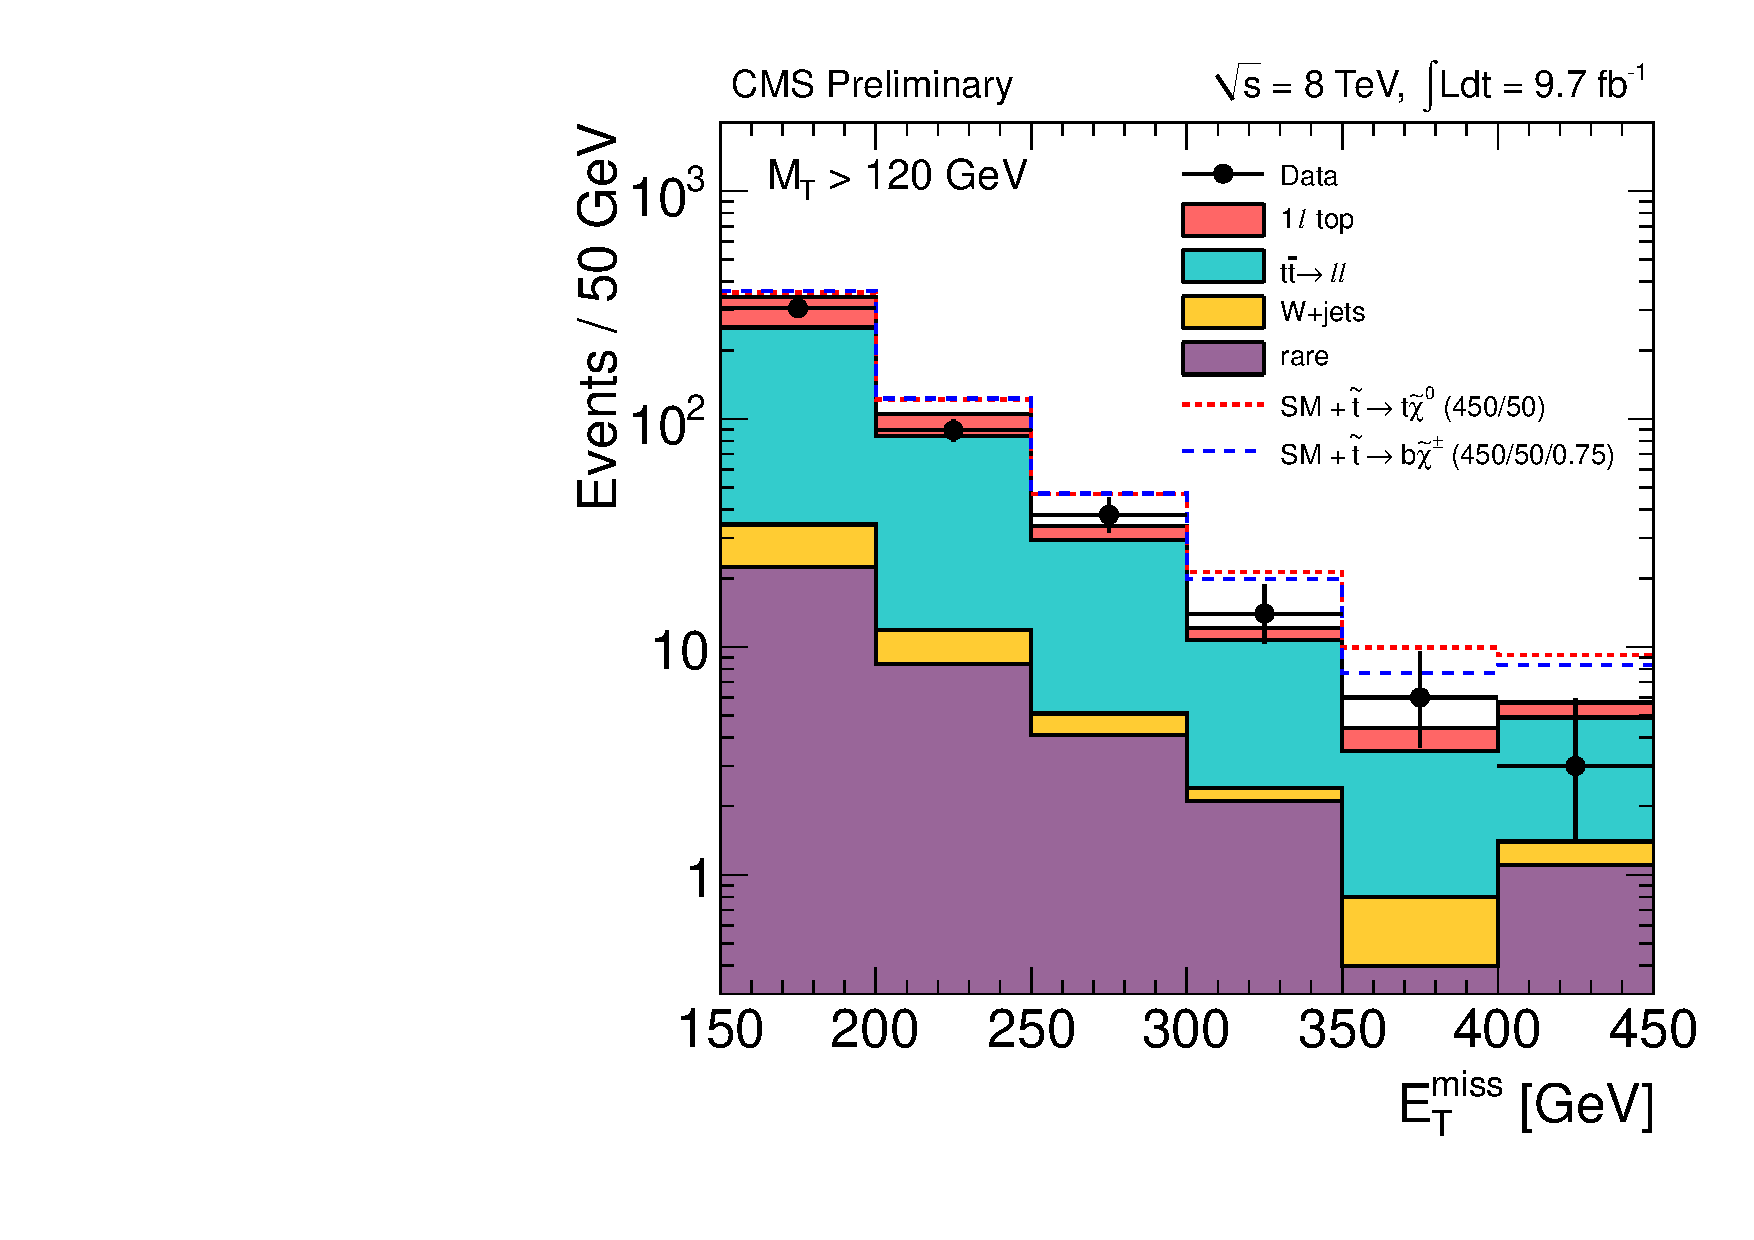
\includegraphics[width=0.4\textwidth]{HCPPlots/stopmet.pdf}
%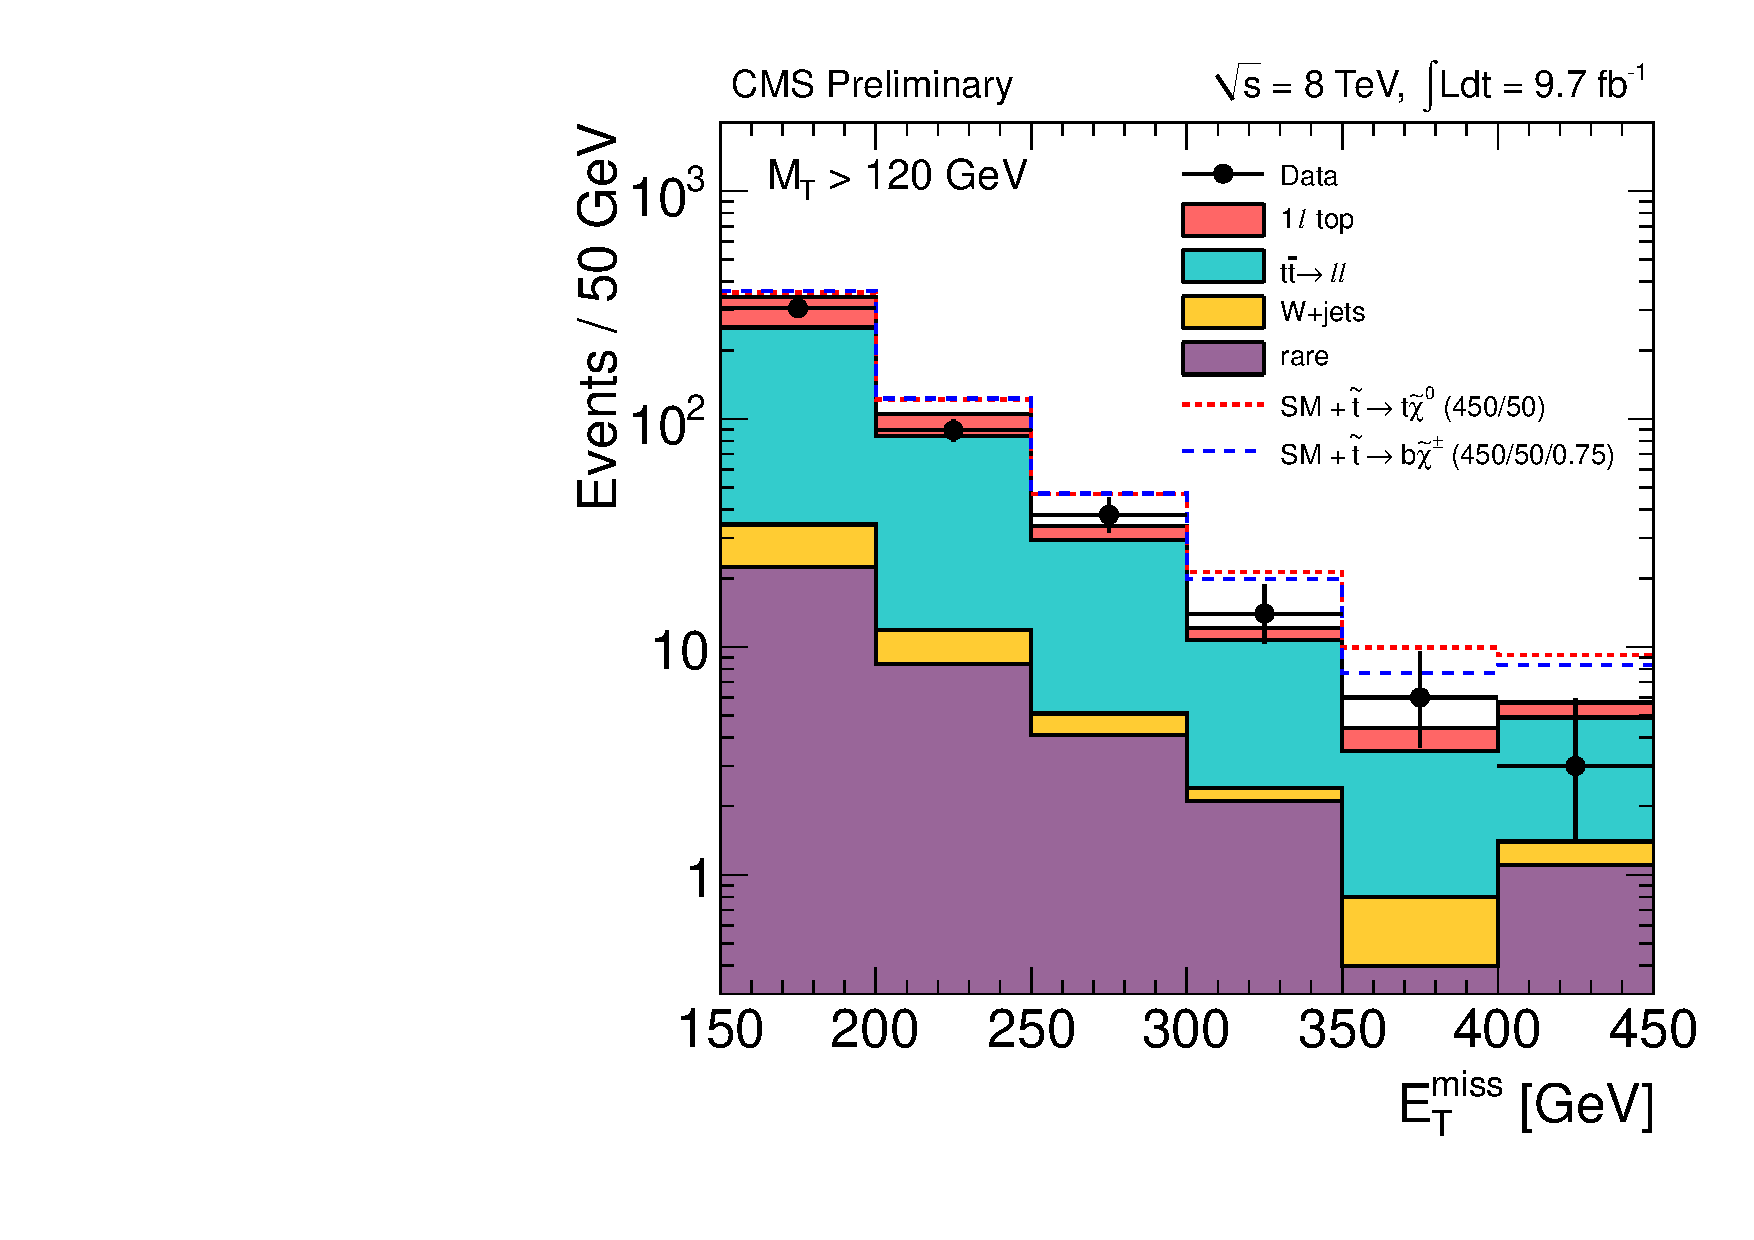
\includegraphics[width=7cm,clip]{HCPPlots/stopmet.pdf}
\caption{The \met\ distribution in data, compared to the sum of expected backgrounds, for the top squark pair search.
Two example signal models are also indicated.}
\label{fig:stop}       % Give a unique label
\end{figure}

%\subsection{Interpretation}

%To interpret the results of our search, we consider two signal scenarios of top squark pair production, followed by the decays
%$\tilde{t}\to t\lsp$ and $\tilde{t}\to b\chip\to b W \lsp$. In the first scenario, the only SUSY particles which participate
%are the top squark and \lsp, and the model can thus be parameterized by the masses of these two particles. In the second case
%the chargino mass is also relevant, and we introduce a third parameter $x$, defined as $m_{\chip} = x m_{\lsp} + (1-x) m_{\tilde{t}}$.
%We consider $x=0.5$ and $x=0.75$ (we do not have sensitivity to the $x=0.25$ scenario).

To interpret the results of our search, we consider top squark pair production where both top squarks decay according to 
$\tilde{t}\to t\lsp$ as depicted in Fig.~\ref{fig:diagrams}(a).
The model is parameterized by the masses of the top squark and \lsp. We place upper limits on the signal
production cross section using, for each model point in the 2-dimensional parameter space, the signal region with the best expected
sensitivity. A region of the parameter space is excluded by comparing these cross section upper limits with the theoretical predictions 
for the signal cross section.
%, computed at next-to-leading order including the resummation of soft gluon emission at 
%next-to-leading-logarithmic
%accuracy (NLO+NLL)~\cite{ref:nlonll}. 
Our results probe top squarks with masses up to 430 GeV. For comparison, the requirement that SUSY
provides a natural solution to the hierarchy problem suggests top squarks with masses not exceeding 500--700 GeV~\cite{ref:naturalsusy}.
We also interpret our results assuming the top squark decays according to $\tilde{t}\to b\chip\to b W \lsp$,
as depicted in Fig.~\ref{fig:diagrams}(b)~\cite{ref:stop}.

The ATLAS experiment has presented a similar search for top squark pairs in the single lepton final state~\cite{ref:atlasstop}.
The constraints from ATLAS on the top squark mass are more stringent than those presented here. The ATLAS model assumes large 
right-handed top quark polarization, while we take the top quark in the $\tilde{t}\to t\lsp$ decay to be unpolarized, 
resulting in a lower signal selection efficiency in our analysis.

\begin{figure}
% Use the relevant command for your figure-insertion program
% to insert the figure file.
\centering
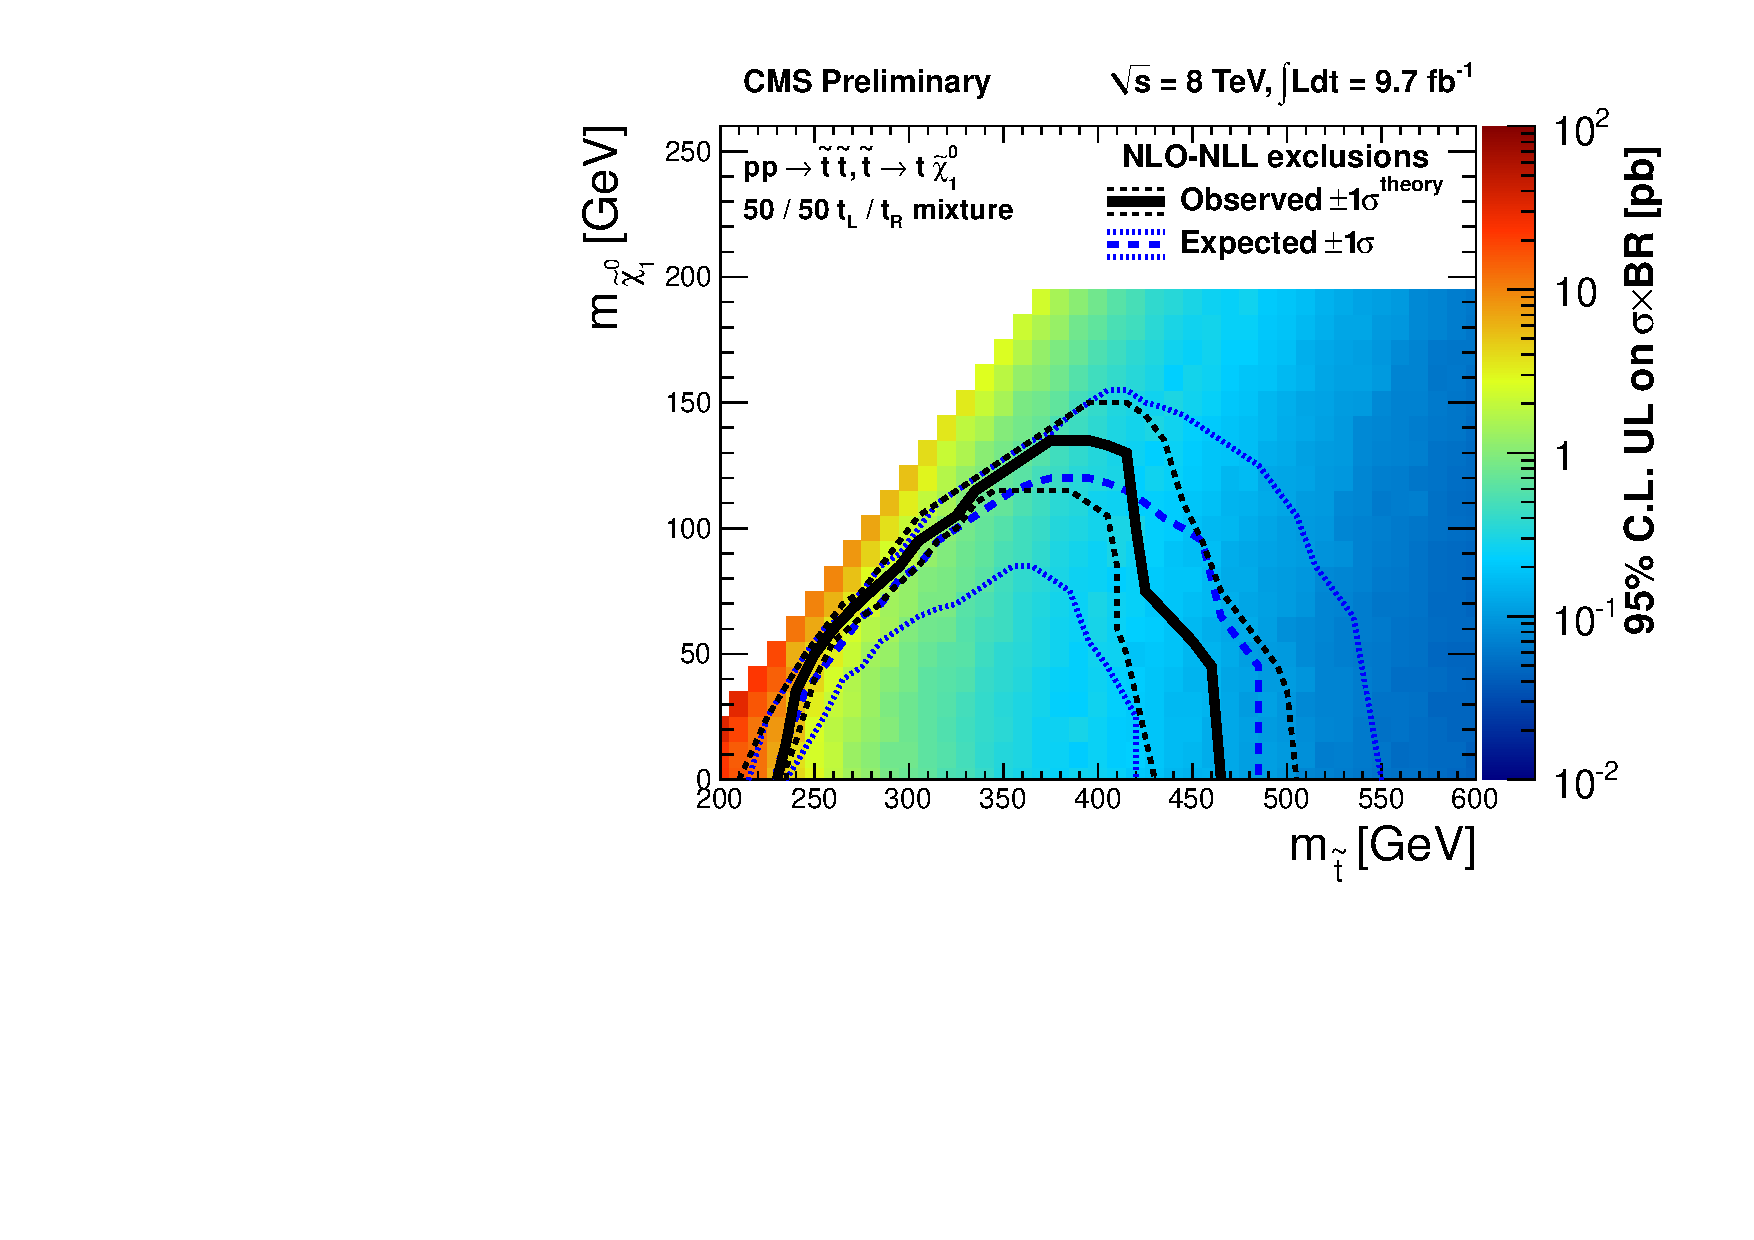
\includegraphics[width=0.5\textwidth]{HCPPlots/stop_interpretation.pdf}
%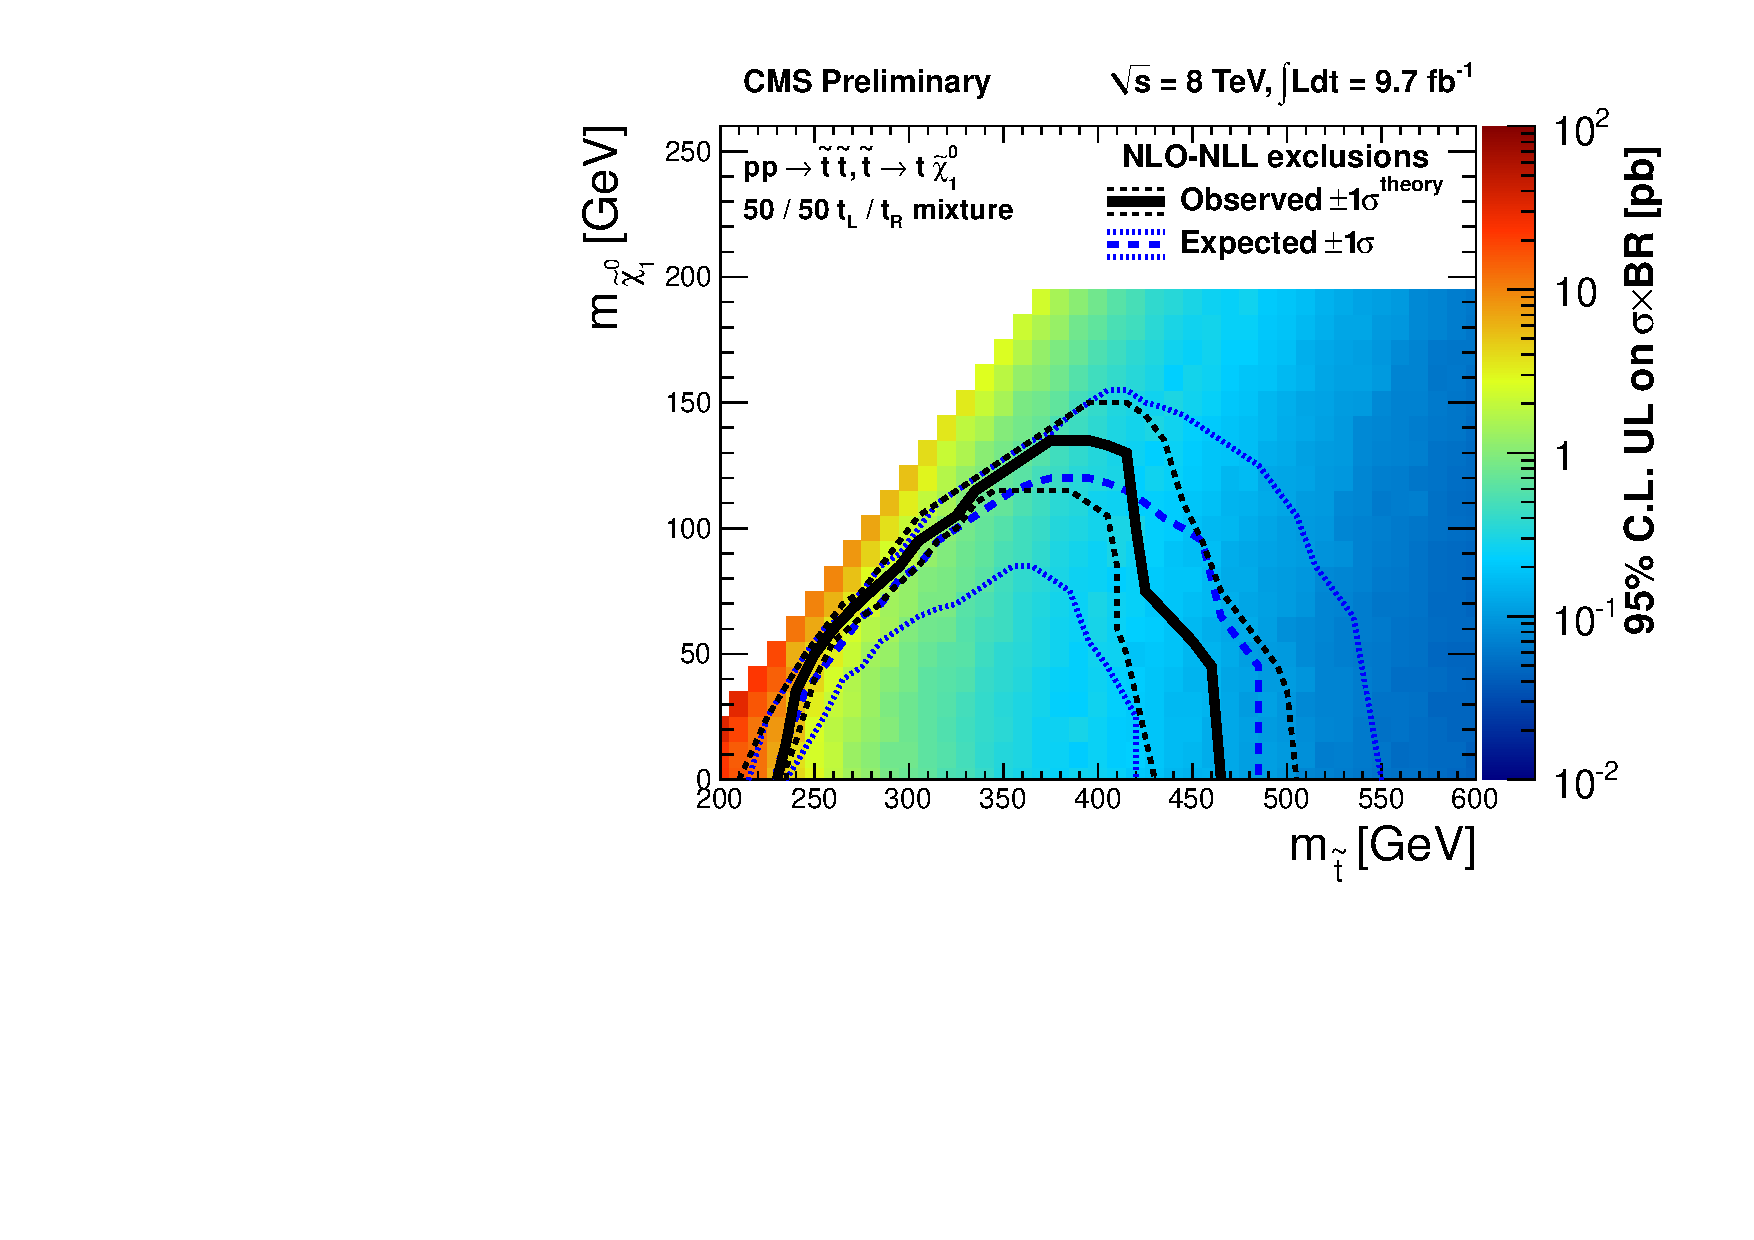
\includegraphics[width=7cm,clip]{HCPPlots/stop_interpretation.pdf}
\caption{Interpretation of the results of the top squark pair search in the $\tilde{t}\to t\lsp$ scenario of 
Fig.~\ref{fig:diagrams}(a). The color scale indicates the cross section upper limits. The solid black contour 
and dashed black contours indicate the observed excluded region and variation in this
excluded region due to the $\pm1\sigma$ uncertainties in the theoretical prediction of the signal cross section. The dashed blue
and dotted blue contours indicate the median and $\pm1\sigma$ expected excluded regions. }
\label{fig:stop_interpretation}       % Give a unique label
\end{figure}
